
\chapter{ನಿಖರ ಸರ್ವೇಗೆ ಶಾಪ ಭೂಮಿಯ ಏರಿಳಿತ ಮತ್ತು ವಕ್ರತೆಯ ಗುಣ}

ಪ್ರಾಥಮಿಕವಾಗಿ ಸರ್ವೇಯಲ್ಲಿ ಎರಡು ವಿಧಗಳಿವೆ. ಒಂದನೆಯದು ಸಮತಲ ಸರ್ವೇ, ಎರಡನೆಯದು ಜೀಯೊಡೆಟಿಕ್​ ಸರ್ವೇ. ಸಮತಲ ಸರ್ವೇ ಎಂದರೆ ಭೂಮಿಯು ಸಮತಲವಾಗಿದೆ ಎಂದು ಬಾವಿಸಿಕೊಂಡು ಮಾಡುವ ಸರ್ವೇ. ನಮ್ಮ ಕೆಡಸ್ಟ್ರಲ್​ ಸರ್ವೇಯನ್ನು ಮಾಡುವಾಗ ಭೂಮಿಯು ಸಮತಲವಾಗಿದೆ ಎಂದು ಭಾವಿಸಿಕೊಂಡು ಸರ್ವೇಯನ್ನು ಮಾಡಲಾಗುತ್ತದೆ. ಆದ್ದರಿಂದ ಕೆಡಸ್ಟ್ರಲ್​ ಸರ್ವೇಯು ಸಮತಲ ಸರ್ವೇಗೆ ಉದಾಹರಣೆಯಾಗಿದೆ. ಕೆಡಸ್ಟ್ರಲ್​ ಸರ್ವೇ ಎಂದರೆ, ಕಂದಾಯ ನಿರ್ಧಾರಕ್ಕೆ ಪ್ರತೀ ಆಸ್ತಿಯ ಗಡಿಯನ್ನು ಮತ್ತು ಅದರ ಮಾಲಿಕತ್ವವನ್ನು ನಿರ್ಧರಿಸಿ, ಕಂದಾಯ ಆಡಳಿತದ ಉದ್ದೇಶಕ್ಕಾಗಿ ಮಾಡುವ ರೆವಿನ್ಯೂ ಗ್ರಾಮದ ಸರ್ವೇ. ಇದು ಒಂದು ಗ್ರಾಮ ವ್ಯಾಪ್ತಿಯ, ಸಣ್ಣ ಪ್ರಮಾಣದ ವಿಸ್ತೀರ್ಣದಲ್ಲಿ ಮಾಡುವ ಸರ್ವೇ. ಈ ಸಂದರ್ಭದಲ್ಲಿ ವಿಲೇಜ್​ ಮ್ಯಾಪನ್ನು ತಯಾರಿಸಲಾಗುತ್ತದೆ. ಸುಮಾರು \enginline{25} ಕಿಲೋಮೀಟರ್​ ಉದ್ದ ಮತ್ತು \enginline{25} ಕಿಲೋಮೀಟರ್​ ಅಗಲದ ಸಣ್ಣ ವಿಸ್ತೀರ್ಣದಲ್ಲಿ ಭೂಮಿಯ ಗೋಳಾಕೃತಿಯ ಸ್ವರೂಪವು ಗಮನಕ್ಕೆ ಬಾರದಷ್ಟು ಚಿಕ್ಕದಾಗಿರುತ್ತದೆ.

ಸರ್ವೇಯ ಎರಡನೆಯ ವಿಧ, ಜಿಯೋಡೆಟಿಕ್​ ಸರ್ವೇ. ಭೂಮಿಯು ನಿಜವಾಗಿಯೂ ಸಮತಲವಾಗಿಲ್ಲ. ಅದು ಗೋಳಾಕಾರವಾಗಿದೆ. ಜಿಯೋಡೆಟಿಕ್​ ಸರ್ವೇಯನ್ನು ಮಾಡುವಾಗ ಭೂಮಿಯ ಗೋಳಾಕೃತಿಯ ಸ್ವರೂಪವನ್ನು ಪರಿಗಣಿಸಲಾಗುತ್ತದೆ. ಜಿಯೋಡೆಟಿಕ್​ ಸರ್ವೇಯು ದೇಶ ವ್ಯಾಪ್ತಿಯ ವಿಶಾಲ ಪ್ರದೇಶದಲ್ಲಿ ಮಾಡುವ ಸರ್ವೇಯಾಗಿದೆ. ಭಾರತದಲ್ಲಿ\break ಲ್ಯಾಂಬ್​ಟನ್​ರವರ ಉದ್ದೇಶಿತ ಗ್ರೇಟ್​ ಟ್ರಿಗನಮಿಟ್ರಿಕಲ್​ ಸರ್ವೇಯು ಜೀಯೊಡೆಟಿಕ್​ ಸರ್ವೇಗೆ ಉತ್ತಮ ಉದಾಹರಣೆ. ಟೋಪೋಗ್ರಫಿಕಲ್​ ಸರ್ವೇಯು ಸಹ ಜೀಯೋಡೆಟಿಕ್​ ಸರ್ವೇಯೇ ಆಗಿದೆ. ಟೋಪೋಗ್ರಫಿಕಲ್​ ಸರ್ವೇ ಎಂದರೆ, ಭೂಮಿಯ ಚಿತ್ರಣವನ್ನು, ಸ್ಥಳ ಸ್ವರೂಪವನ್ನು ನೀಡುವ ಸರ್ವೇ. ಟೋಪೋಗ್ರಫಿಕಲ್​ ಮ್ಯಾಪನ್ನು ಈ ಸಂದರ್ಭದಲ್ಲಿ ತಯಾರಿಸಲಾಗುತ್ತದೆ. ಈ ಟೋಪೋ ಮ್ಯಾಪುಗಳಲ್ಲಿ ಅಕ್ಷಾಂಶ ರೇಖಾಂಶ ರೇಖೆಗಳು, ಕಾಂಟೂರ್​ ರೇಖೆಗಳು, ಸರಾಸರಿ ಸಮುದ್ರ ಮಟ್ಟ ಈ ವಿವರಗಳಿರುತ್ತವೆ.

\begin{center}
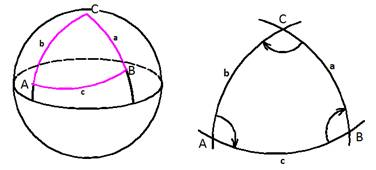
\includegraphics[scale=0.55]{"images/image001.jpg"}
\end{center}

ಭೂಮಿಯು ಏರು ತಗ್ಗು, ಬೆಟ್ಟ ಕಣಿವೆಗಳಿಂದ ಕೂಡಿದೆ. ಈ ಏರು ತಗ್ಗುಗಳನ್ನು, ಒಂದು ಸಮತಲದ ಮೇಲೆ ಪ್ರಕ್ಷೇಪಿಸಿಕೊಂಡು, ಅಳತೆಗಅಳನ್ನು ಪಡೆಯಬೇಕು. ನಂತರ, ಜಾಮಿತಿಯ ಮತ್ತು ಟ್ರಿಗನಮಿಟ್ರಿಯ ತತ್ವಗಳನ್ನು ಆ ಅಳತೆಗಳಿಗೆ ಅನ್ವಯಿಸಿ, ಲೆಕ್ಕಾಚಾರ ಮಾಡಿ, ನಕ್ಷೆ ತಯಾರಿಸುವುದು ಸರ್ವೇಯ ಕ್ರಮ. ಇದು ಸೈದ್ಧಾಂತಿಕವಾಗಿ, ಗಣಿತ ಲೆಕ್ಕಚಾರದಲ್ಲಿ ಯಾವುದೇ ಸಮಸ್ಯೆಯೂ ಅಲ್ಲ. ಆದರೆ ಸಮಸ್ಯೆ ಮತ್ತು ಸಂಕೀರ್ಣತೆ ಇರುವುದು ಭೂಮಿಯು ಏರು ತಗ್ಗುಗಳಿಂದ ಕೂಡಿರುವುದರ ಜೊತೆಗೆ ಅದು ಗುಂಡಾಗಿರುವುದು. ರೇಖಾ ಗಣಿತದ ಪ್ರಕಾರ, ತ್ರಿಭುಜದಲ್ಲಿ ಮೂರು ಕೋನಗಳಿರುತ್ತವೆ ಮತ್ತು ಆ ಮೂರು ಕೋನಗಳ ಮೊತ್ತವು \enginline{1800} ಇರುತ್ತದೆ. ಚಿತ್ರದಲ್ಲಿ ತೋರಿಸಿದಂತೆ, ಭೂಮಿಯ ಮುಖದ ಮೇಲೆ ಯಾರಾದರೂ ಒಂದು ದೊಡ್ಡ ತ್ರಿಭುಜವನ್ನು ರಚಿಸಿದರೆ, ಆ ತ್ರಿಭುಜದ ಮೂರು ಕೋನಗಳ ಮೊತ್ತವು \enginline{1800} ಆಗಿರುವುದಿಲ್ಲ. ಏಕೆಂದರೆ, ಭೂಮಿಯ ಗುಂಡಾದ ಮುಖದ ಮೇಲೆ, ತ್ರಿಭುಜದ ಬಾಹುಗಳು, ನೇರ ರೇಖೆಗಳಾಗಿರುವುದಿಲ್ಲ. ಅವುಗಳು ತುಸು ಹೊರ ಬಾಗಿರುವುದರಿಂದ, ಮೂರು ಕೋನಗಳ ಮೊತ್ತವು \enginline{1800} ಗಿಂತ ತುಸು ಹೆಚ್ಚಿರುತ್ತದೆ. ಈ ವ್ಯತ್ಯಾಸವನ್ನು ‘ಸ್ಪೆರಿಕಲ್​ ಎಕ್ಸಸ್​’ ಅಥವಾ ‘ಗೋಳೀಯ ಹೆಚ್ಚುವರಿ’ ಎನ್ನುತ್ತಾರೆ. ಭೂಮಿಯ ಮೇಲಿನ, ಯಾವುದೇ ರೇಖೆಯು ಸರಳ ರೇಖೆಯಾಗಿರದೇ, ಅದು ಗೋಳದ ಮೇಲಿನ ವಕ್ರ ರೇಖೆಯಾಗಿರುವುದರಿಂದ, ಸ್ವಲ್ಪ ದೊಡ್ಡದಾದ ಅಳತೆಯಲ್ಲಿ ಈ ಗೋಳೀಯ ಹೆಚ್ಚುವರಿಯನ್ನು ಕಳೆಯಬೇಕು. ಭೂಮಿಯಲ್ಲಿನ ಏರು ತಗ್ಗುಗಳು ಮತ್ತು ಅದರ ಗೋಳಿಯ ಮೈ ಆಕಾರವು ಲೆಕ್ಕಾಚಾರಕ್ಕೆ ಹೊಸ ಆಯಾಮವನ್ನು ಕೊಡುತ್ತದೆ. ಭೂಮಿಯ ಈ ಏರುತಗ್ಗು ಮತ್ತು ಅದರ ಗೋಳಾಕಾರದ ಗುಣ ಸ್ವರೂಪವು ಯಾವುದೇ ನಿಖರವಾದ ಸರ್ವೇಗೆ ಒಂದು ಶಾಪವೇ ಆಗಿದೆ. ಈ ಕಾರಣಕ್ಕೆ, ಭೂಮಿಯ ಮೇಲೆ ಮಾನವ ಮಾಡಿದ ಯಾವುದೇ ಅಳತೆಯು, ಸಂಪೂರ್ಣ ನಿಖರತೆಯಿಂದ ಕೂಡಿರುವುದಿಲ್ಲ. ಒಂದಷ್ಟು ದೋಷವಿದ್ದೇ ಇರುತ್ತದೆ.

\begin{center}
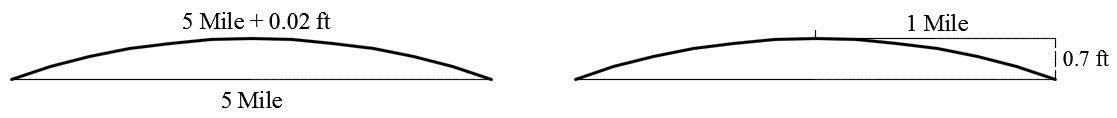
\includegraphics[scale=0.5]{"images/image002.jpg"}
\end{center}

ಭೂಮಿಯ ಮೇಲಿನ ಐದು ಮೈಲು ಅಂತರದಲ್ಲಿ, ವೃತ್ತ ಕಂಸ ಮತ್ತು ರೇಖಾ ಖಂಡ ಇವುಗಳ ಅಂತರದ ವ್ಯತ್ಯಾಸವು ಕೇವಲ \enginline{0.02} ಅಡಿಯಷ್ಟಿರುತ್ತದೆ. ಭೂಎಲಿಪ್ಸಾಯಿಡ್​ಗೆ ಒಂದು ಸ್ಪರ್ಶಕ ರೇಖೆ ಎಳೆದರೆ, ಅದು ಒಂದು ಮೈಲು ಅಂತರದಲ್ಲಿ \enginline{0.7} ಅಡಿಯಷ್ಟು ಹೊರಳುತ್ತದೆ. \enginline{75} ಚದರ ಮೈಲು ತ್ರಿಭುಜದಲ್ಲಿ ಅಂದರೆ, ತಲಾ \enginline{13} ಮೈಲು ಇರುವ ಸಮಬಾಹು ತ್ರಿಭುಜದಲ್ಲಿ, ಮೂರು ಎಲಿಪ್ಸಾಯಿಡ್​ ಕೋನಗಳ ಮೊತ್ತ ಮತ್ತು ಮೂರು ಸಮತಲ ಕೋನಗಳ ಮೊತ್ತ ಇವುಗಳ ವ್ಯತ್ಯಾಸವು ಕೇವಲ ಒಂದು ಸೆಕೆಂಡಿನಷ್ಟು ಮಾತ್ರ. ಇದರರ್ಥ ವಿಶಾಲ ಪ್ರದೇಶದ ಅಳತೆಗಳಲ್ಲಿ ಮಾತ್ರ ವಕ್ರತೆ ಪರಿಗಣಿತವಾಗುತ್ತದೆ. ಕೆಲವು ನೂರು ಚದುರ ಮೈಲಿಗಳ ಸಣ್ಣ ಸರ್ವೇಯಲ್ಲಿ ಭೂಮಿಯ ವಕ್ರತೆಯಿಂದ ಉಂಟಾಗುವ ದೋಷವು ಅತಿ ಅಲ್ಪ ಪ್ರಮಾಣದ್ದು, ಲೆಕ್ಕಕ್ಕೆ ಬಾರದಷ್ಟು ಚಿಕ್ಕದು. ಅದನ್ನು ಕಡೆಗಣಿಸಬಹುದು. ಸರ್ವೇಯ ಕೊನೆ ತುದಿಗಳಲ್ಲಿ ರೇಖಾಂಶ, ಅಕ್ಷಾಂಶಗಳ ನಿಖರ ವೀಕ್ಷಣೆಯಿಂದ ಆ ದೋಷವನ್ನು ಸರಿ ಸಮಾನವಾಗಿ ಅಂದಾಜಿನಲ್ಲಿ ಹಂಚಿಹಾಕಬಹುದು. ಇದು ಕರ್ನಲ್​ ಮೆಕೆಂಜಿಯವರು ತಮ್ಮ ಮೈಸೂರು ಸರ್ವೇ ಕಾರ್ಯದಲ್ಲಿ ಮಾಡಿದ ಕ್ರಮ. ಆದರೆ ಸಾವಿರಾರು ಚದುರ ಮೈಲು ವಿಸ್ತೀರ್ಣದ, ವಿಸ್ತಾರವಾದ ಸರ್ವೇಯಲ್ಲಿ ಈ ಕ್ರಮವು ತೃಪ್ತಿಕರವಾದದ್ದು ಅಲ್ಲ. ಏಕೆಂದರೆ ದೋಷದ ಪ್ರಮಾಣವು ಸಂಚಿತಗೊಂಡು, ಇಮ್ಮಡಿಯಾಗಿ ಮುಮ್ಮಡಿಯಾಗಿ ಬೆಳೆದು ಇಡೀ ಸರ್ವೇಯನ್ನು ದೋಷಮಯವಾಗಿ ಮಾಡಿಬಿಡುತ್ತದೆ. ಪ್ರಾಚೀನ ಭೂಗೋಳ ತಜ್ಞರು ಇದಕ್ಕೆ ಸೂಚಿಸಿದ ಸರಳ ಪರಿಹಾರವೆಂದರೆ, ಗೋಳಾಕಾರದ ಭೂಮಿಯ ತ್ರಿಜ್ಯ ಹಾಗೂ ಸುತ್ತಳತೆಯನ್ನು ಕಂಡುಹಿಡಿದು, ಭೂ ವಕ್ರತೆಗೆ ಒಂದು ಮಾದರಿ ನಿಯತಾಂಕಅವನ್ನು ಲೆಕ್ಕಾಚಾರದಿಂದ ಕಂಡುಹಿಡಿದು, ತ್ರಿಭುಜೀಕರಣದ ಉದ್ದಕ್ಕೂ ಅದನ್ನು ಅನ್ವಯಿಸುವುದು.

ನಿಖರ ಅಳತೆಗೆ ಭೂಮಿಯ ಏರುತಗ್ಗು ಮತ್ತು ಗೋಳಾಕೃತಿಯ ಸ್ವರೂಪವು ಒಂದು ಸಮಸ್ಯೆ. ಇದರಲ್ಲಿ ಇನ್ನೂ ಸಂಕೀರ್ಣವಾದ ಸಮಸ್ಯೆ ತಲೆದೋರುತ್ತದೆ. ಭೂಮಿ ಗುಂಡಾಗಿದ್ದರೂ ಅದು ನಿಖರವಾಗಿ ಗೋಳಾಕಾರದಲ್ಲಿ ಇಲ್ಲ. \enginline{17}ನೇ ಶತಮಾನದ ಖಗೋಳ ವಿಜ್ಞಾನಿಗಳು, ಭೂಗೋಳ ತಜ್ಞರು ಮತ್ತು ಸರ್ವೇಯರುಗಳು ‘ಭೂಮಿಯು ನಿಜವಾಗಿ ಪರಿಪೂರ್ಣವಾದ ಗೋಳ ಆಗಿಲ್ಲ. ಅದು ಒಂದು ‘ಗೋಳಾಭ’ (ಅಥವಾ ‘ಸ್ಪೆರಾಯ್ಡ್​’ ಅಥವಾ ‘ಎಲಿಪ್ಸಾಯಡ್​’) ಆಗಿದೆ’ ಎಂದರು. ‘ಗೋಳಾಭ’ ಎಂದರೆ, ಗೋಳದ ಒಂದು ರೀತಿ ಅದು ಅಷ್ಟೆ. ಗೋಳದ ಯಾವ ಒಂದು ರೀತಿ? ಈ ಪ್ರಶ್ನೆಯು, ಬಹು ಸಂಕೀರ್ಣವಾದ ಚರ್ಚೆಯ ವಿಷಯ. ಪಾರ್ಶ್ವದಲ್ಲಿ ಸಮತಟ್ಟಾಗಿರುವ, ನೆಟ್ಟಗೆ ನಿಲ್ಲಿಸಿದ ಮೊಟ್ಟೆಯ ರೀತಿಯಾ ಅಥವಾ ನೆತ್ತಿಯ ಮೇಲೆ ಮಟ್ಟವಾಗಿರುವ ದ್ರಾಕ್ಷಿ ಹಣ್ಣಿನ ರೀತಿಯಾ? ಸರಿ, ಮಟ್ಟವಾಗಿದೆ ಅಂದುಕೊಂಡರೂ ಎಷ್ಟು ಮಟ್ಟವಾಗಿದೆ? ಇದು ನಿಜವಾದ ಸಮಸ್ಯೆ.

ಸಮಾಧಾನಕರ ವಿಷಯವೆಂದರೆ, ಲ್ಯಾಂಬ್​ಟನ್​ರವರ ಕಾಲದಲ್ಲಿ ಈ ಕೋಳಿ ಮೊಟ್ಟೆ ವರ್ಸಸ್​ ದ್ರಾಕ್ಷಿ ಹಣ್ಣಿನ ಪ್ರಶ್ನೆ ಬಗೆಹರಿದಿತ್ತು. \enginline{1730}ರಲ್ಲಿ ಈ ವಿಶೇಷ ಕಾರ್ಯಾಕ್ಕಾಗಿಯೇ ಎರಡು ವಿಶೇಷ ಕಾರ್ಯ ತಂಡಗಳನ್ನು ಫ್ರಾನ್ಸ್​ನಿಂದ ಕಳುಹಿಸಲಾಗಿತ್ತು. ಒಂದು ತಂಡ, ಈಗ ಇಕ್ವೆಡಾರ್​ ಎಂದು ಕರೆಯಲಾಗುವ ಸಮಭಾಜಕ ವೃತ್ತದ ಭಾಗಅಕ್ಕೆ. ಇನ್ನೊಂದು ತಂಡ ಲ್ಯಾಪ್​ಲ್ಯಾಂಡ್​ನ ಆರ್ಕ್ಟಿಕ್​ ವೃತ್ತದ ಭಾಗಕ್ಕೆ. ಪ್ರತಿ ತಂಡದ ಕಾರ್ಯ ಏನೆಂದರೆ, ಸುಮಾರು ಇನ್ನೂರು ಮೈಲು ಅಳತೆಯ ಚಿಕ್ಕ ಆರ್ಕ್ ಅಥವಾ ವೃತ್ತ ಕಂಸವನ್ನು ರೇಖಾಂಶ (ಮೆರಿಡಿಯನಲ್​) ನೇರದಲ್ಲಿ ರಚಿಸುವುದು. ವೃತ್ತ ಕಂಸದಅ ಕೊನೆ ತುದಿಗಳ ಸ್ಥಾನಗಳನ್ನು, ಅವುಗಳ ನಡುವಿನ ಕೋನೀಯ ಅಂತರವನ್ನು, ನಿಖರ ಖಗೋಳ ವೀಕ್ಷಣೆಯಿಂದ ಕಂಡುಹಿಡಿದು, ನಿಗಧಿ ಮಾಡುವುದು. ಈ ಮೆರಿಡಿಯನಲ್​ ಆರ್ಕ್ ರೇಖೆಯ ಉದ್ದವನ್ನು, ದಕ್ಷಿಣೋತ್ತರ ಟ್ರೈಯಾಂಗ್ಯುಲೇಶನ್​ನಿಂದ, ನಿಖರ ಬೇಸ್​ಲೈನ್​ ಅಳತೆ ಮಾಡಿ ಕಂಡುಹಿಡಿಯುವುದು. ನಂತರ ಒಂದು ಡಿಗ್ರಿ ಆರ್ಕ್ ಮೇಲಿನ ನಿಜವಾದ ಪ್ರಾಯೋಗಿಕ ಅಂತರ ಏನು ಎಂದು ಲೆಕ್ಕಾಚಾರ ಮಾಡುವುದು. ಒಂದು ಡಿಗ್ರಿ ಆರ್ಕ್ನ ಅಂತರ ಏನು ಎಂದು ಕಂಡುಹಿಡಿಯುವುದೇ ಎರಡೂ ತಂಡಗಳ ಉದ್ದೇಶಿತ ಮುಖ್ಯವಾದ ಗುರಿಯಾಗಿತ್ತು. ಈ ಪ್ರಾಯೋಗಿಕ ವಿಶೇಷ ಕಾರ್ಯದ ಬೇಸ್​ ಲೈನ್​ ಅಳತೆ, ಟ್ರೈಯಾಂಗ್ಯುಲೇಷನ್​ ಕಾರ್ಯ, ನಕ್ಷತ್ರ ವೀಕ್ಷಣೆ ಇವುಗಳೆಲ್ಲವನ್ನೂ ನಿಖರಾತಿ ನಿಖರವಾಗಿ ನಿರ್ವಹಿಸಬೇಕು. ಇವುಗಳೆಲ್ಲವೂ ಭಾರೀ ಸಮಯ ತೆಗೆದುಕೊಳ್ಳುವ ಕಾರ್ಯಗಳು. ಇಕ್ವೆಡಾರ್​ನ ತಂಡವು ಈ ಉದ್ದೇಶಿತ ಫಲಿತಾಂಶ ಪಡೆಯಲು \enginline{9} ವರ್ಷ ಕಾರ್ಯ ನಿರ್ವಹಿಸಬೇಕಾಯಿತು.

ಹೆಚ್ಚು ಶ್ರಮವಿಲ್ಲದೆ, ಈ ಎರಡೂ ತಂಡದ ಬಹು ಶ್ರಮದ ಪ್ರಾಯೋಗಿಕ ಫಲಿತಾಂಶವನ್ನು ಒಂದರ ಪಕ್ಕದಲ್ಲಿ ಒಂದನ್ನು ಇಟ್ಟು ಹೋಲಿಸಿ ನೋಡಲಾಯಿತು. ಈ ಕಾರ್ಯಾಚರಣೆಯ ಫಲಿತಾಂಶವೆಂದರೆ, ಈಕ್ವೆಡಾರ್​ನಲ್ಲಿ ಒಂದು ಡಿಗ್ರಿ ಉದ್ದವು \enginline{110} ಕಿಲೊಮೀಟರ್​ ಇತ್ತು.\break ಲ್ಯಾಪ್​ಲ್ಯಾಂಡ್​ನಲ್ಲಿ ಒಂದು ಡಿಗ್ರಿ ಉದ್ದವು \enginline{111} ಕಿಲೊಮೀಟರ್​ ಇತ್ತು. ಅಂದರೆ, ಒಂದು ಡಿಗ್ರಿ ಅಕ್ಷಾಂಶದ ಮೇಲಿನ ಅಳತೆಯು, ಸಮಭಾಜಕ ಮತ್ತು ಧೃವ ಪ್ರದೇಶಗಳಲ್ಲಿ ಒಂದು ಕಿಲೋ ಮೀಟರ್​ನಷ್ಟು ವ್ಯತ್ಯಾಸ ಇತ್ತು. ಸಮಭಾಜಕದಲ್ಲಿ ಅಕ್ಷಾಂಶ ರೇಖೆಗಳು ಒತ್ತೊತ್ತಾಗಿವೆ ಹಾಗೂ ಧೃವಪ್ರದೇಶದಲ್ಲಿ ಅವುಗಳು ವಿರಳವಾಗಿವೆ. ಅಂದರೆ ಭೂಮಿಯ ಮೇಲ್ಮೈ ಸಮಭಾಜಕದಲ್ಲಿ ಹೆಚ್ಚು ವೃತ್ತಾಕಾರವಾಗಿದೆ ಮತ್ತು ದೃವಪ್ರದೇಶದಲ್ಲಿ ಚಪ್ಪಟೆಯಾಗಿದೆ. ಅಂದರೆ, ದ್ರಾಕ್ಷಿ ಹಣ್ಣೇ ಸ್ಪರ್ದೆಯಲ್ಲಿ ಗೆದ್ದು, ತನ್ನ ಪ್ರತಿಸ್ಪರ್ದಿ ಕೋಳಿ ಮೊಟ್ಟೆಯನ್ನು ಕೂದಲೆಅಳೆ ಅಂತರದಲ್ಲಿ ಸೋಲಿಸಿತ್ತು. ಭೂಮಿಯು ದೃವಪ್ರದೇಶದಲ್ಲಿ ಚಪ್ಪಟೆಯಾಗಿರುವ ಒಂದು ಗೋಳಾಭ ಅಥವಾ ಸ್ಪೆರಾಯ್ಡ್​ ಆಗಿರುವುದು ದೃಢಪಟ್ಟಿತು.

